\chapter{Systembeskrivelse}\label{ch:Systembeskrivelse}
Systemet BargainBarter er en Webapplikation, der hostes på \url{http://10.29.0.30/BargainBarter} på en af AU's servere på deres netværk. Denne hjemmeside tilbyder besøgende at oprette sig som bruger, oprette og bytteannoncer og chatte med andre brugere af systemet. 
Kernefunktionaliteten af BargainBarter er at kunne oprette en bytteannonce, med det formål at bytte den med en andens brugers ejendel. Når annoncen er oprettet kan den af andre brugere ses i det samlede overblik over annoncer på forsiden. På forsiden kan der klikkes ind på annoncen for nærmere/flere detaljer. 
Systemet skal igennem annoncen præsentere brugeren for annnoncens lokation, brugerens rating og evt. kommentarer til annoncen.
Systemet skal have et indbygget chat-modul, så brugere kan kommunikere sammen i real-tid om byttehandler mm.
%Herfra har en bruger adgang til informationer om sted/adresse på den tilhørende bruger på bytteannoncen, afstand til den tilhørende bruger, offentlige kommentarer på annoncen, den tilhørende brugers byttehistorik og vurderinger fra andre brugere på baggrund af tidligere byttehandler.
%Brugeren har tilgang til et fælles chatrum, hvor man evt. kan skrive om tid og sted for byttehandlen. \\

\noindent En rigt billede, der illustrer systemets primære funktionalitet og formål kan ses på figur \ref{fig:rigbillede} hvor et simpel byttescenarie demonstreres.

\begin{figure}[H]
	\centering
	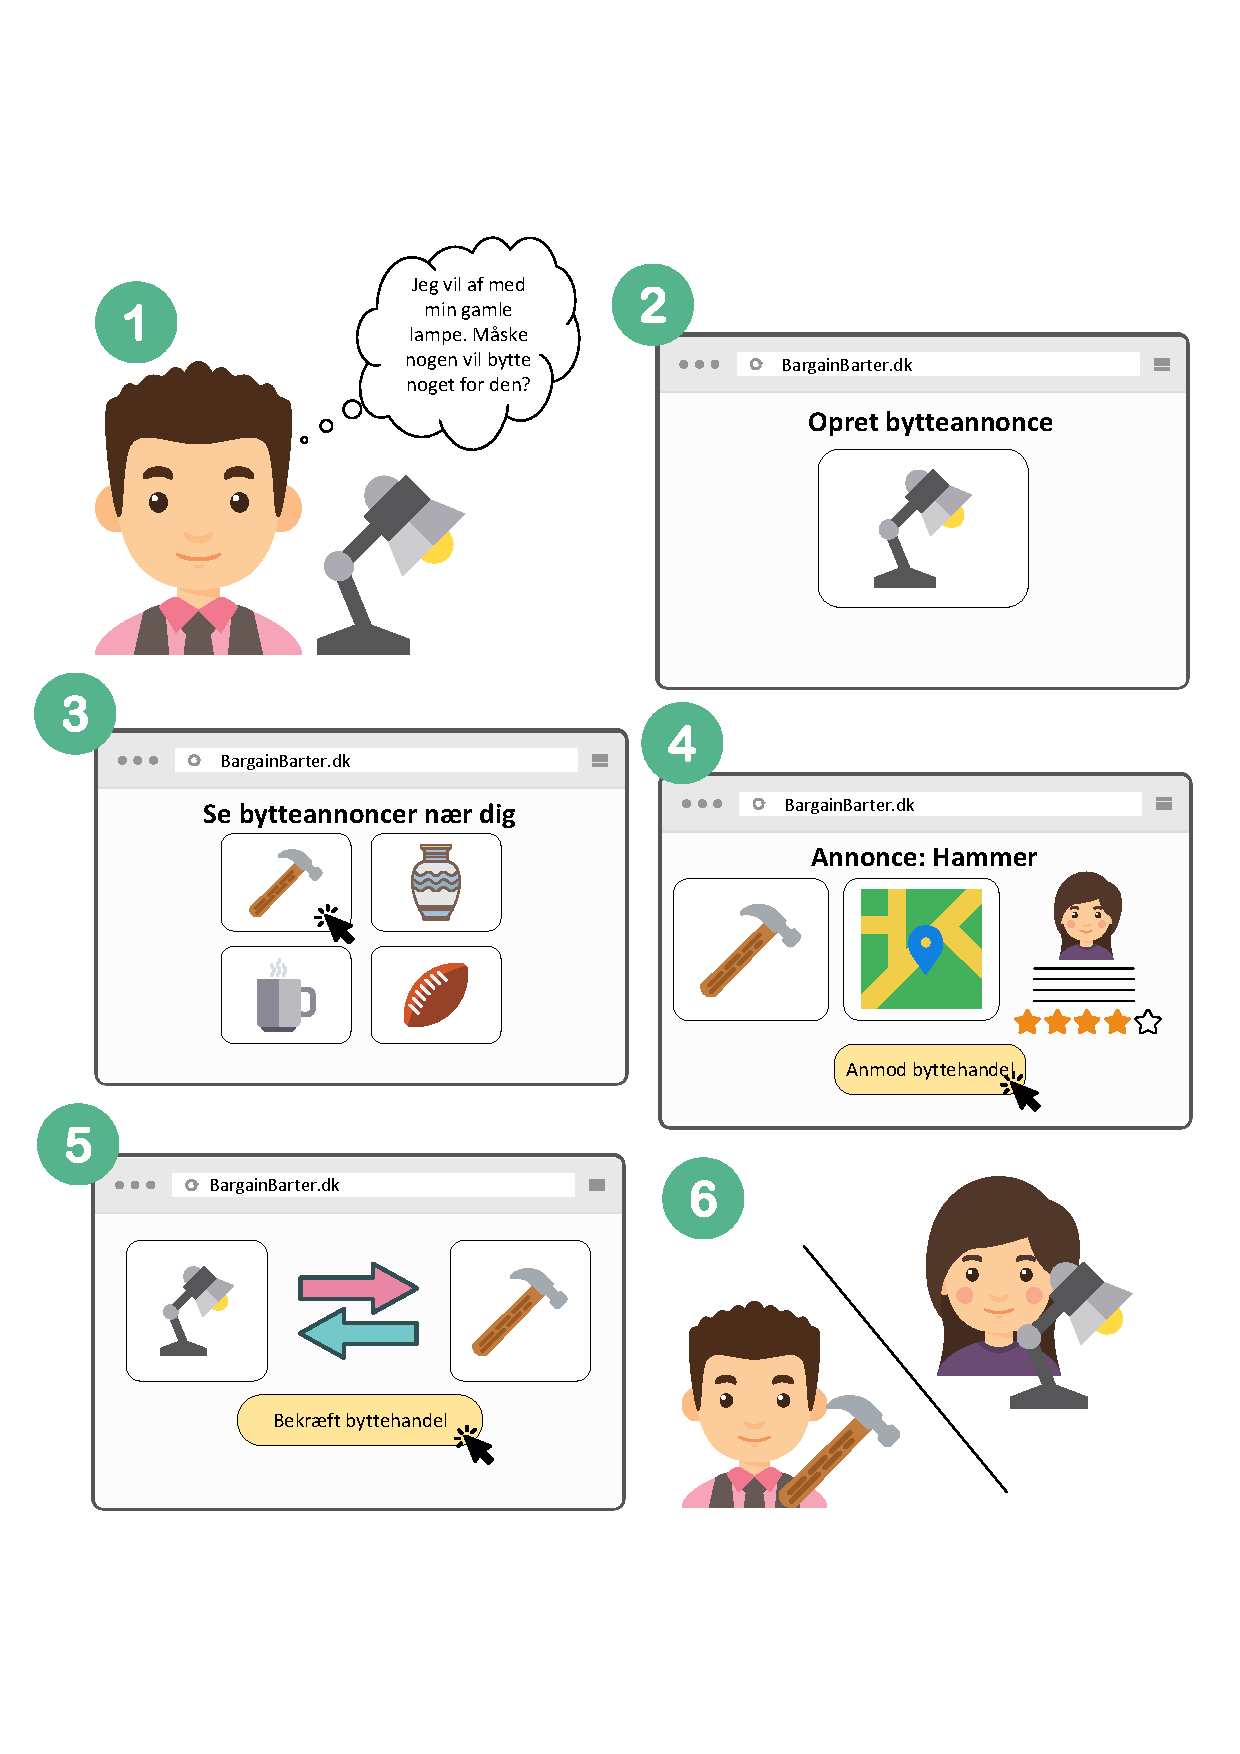
\includegraphics
	[width=140mm]{figures/rigtbillede_version1.pdf}
	\caption{Rigt billede}
	\label{fig:rigbillede}
\end{figure} 



På figur \ref{fig:rigbillede} ses det, at byttehandlerne enten bekræftes eller afvises  direkte i systemet. De fysiske byttehandler foregår dog uden om systemet, og brugeren skal derfor selv udføre handlen for at få værdi af systemet. 